\documentclass[11pt,aspectratio=169]{beamer}
\usepackage[utf8]{inputenc}
\usepackage[T1]{fontenc}
\usepackage{graphicx}
\usepackage{mathtools}
\usepackage{tikz}
\usetikzlibrary{shapes.geometric,arrows.meta,positioning,fit,backgrounds,calc}
\usepackage{booktabs}
\usepackage{array}
\usepackage{multirow}
\usepackage[table]{xcolor}
\usepackage{hyperref}

\usetheme{default}
\usefonttheme{professionalfonts}

% ---------------- COLOUR PALETTE ----------------
\definecolor{navyDeep}{RGB}{110,45,58}
\definecolor{navyMid}{RGB}{168,78,86}
\definecolor{tealAccent}{RGB}{212,166,88}
\definecolor{rustAccent}{RGB}{52,142,126}
\definecolor{paperGrey}{RGB}{247,243,238}
\definecolor{lineGrey}{RGB}{214,204,198}

\setbeamercolor{structure}{fg=navyMid}
\setbeamercolor{frametitle}{bg=navyDeep, fg=white}
\setbeamercolor{title}{bg=navyDeep, fg=white}
\setbeamercolor{item}{fg=tealAccent}
\setbeamercolor{block title}{bg=navyMid, fg=white}
\setbeamercolor{block body}{bg=paperGrey, fg=black}
\setbeamercolor{block title alerted}{bg=rustAccent, fg=white}
\setbeamercolor{block body alerted}{bg=rustAccent!8, fg=black}
\setbeamercolor{caption name}{fg=navyMid}

\setbeamertemplate{frametitle}{%
  \nointerlineskip%
  \begin{beamercolorbox}[wd=\paperwidth,ht=3.1ex,dp=1.5ex,leftskip=0.55cm]{frametitle}%
    \usebeamerfont{frametitle}\insertframetitle%
  \end{beamercolorbox}%
  \nointerlineskip%
  \begin{beamercolorbox}[wd=\paperwidth,ht=0.6mm,dp=0mm]{}%
    \color{tealAccent}\rule{\paperwidth}{0.6mm}%
  \end{beamercolorbox}%
  \vskip0.35cm%
}
\setbeamerfont{frametitle}{series=\bfseries,size=\large}

\setbeamercolor{footL}{bg=navyDeep, fg=white}
\setbeamercolor{footC}{bg=navyMid,  fg=white}
\setbeamercolor{footR}{bg=navyDeep, fg=white}

\setbeamertemplate{footline}{%
  \leavevmode%
  \hbox{%
    \begin{beamercolorbox}[wd=.30\paperwidth,ht=3.0ex,dp=1.5ex,left]{footL}%
      \hspace*{0.55cm}\usebeamerfont{footline}\scriptsize CSE, IIIT Vadodara
    \end{beamercolorbox}%
    \begin{beamercolorbox}[wd=.50\paperwidth,ht=3.0ex,dp=1.5ex,center]{footC}%
      \usebeamerfont{footline}\scriptsize Predictive Sprint Planning \& Delivery Risk Tool
    \end{beamercolorbox}%
    \begin{beamercolorbox}[wd=.20\paperwidth,ht=3.0ex,dp=1.5ex,right]{footR}%
      \usebeamerfont{footline}\scriptsize\insertframenumber\,/\,\inserttotalframenumber\hspace*{0.4cm}
    \end{beamercolorbox}%
  }%
  \vskip0pt%
}

\setbeamertemplate{navigation symbols}{}
\setbeamertemplate{itemize item}{\color{tealAccent}\raisebox{0.15ex}{\scriptsize$\blacksquare$}}
\setbeamertemplate{itemize subitem}{\color{navyMid}\textendash}
\setbeamertemplate{enumerate item}{\color{white}\colorbox{navyMid}{\footnotesize\insertenumlabel}}
\setbeamertemplate{blocks}[rounded][shadow=false]
\setbeamersize{text margin left=0.75cm, text margin right=0.75cm}
\hypersetup{colorlinks=true, linkcolor=navyMid, urlcolor=navyMid}

% ---------------- HELPERS ----------------
\newcommand{\panel}[2][0.86]{%
  \begin{center}%
  \begin{tikzpicture}
    \node[fill=navyMid, rounded corners=8pt, text=white, align=left,
          text width=#1\textwidth-12pt, inner sep=6pt] {#2};
  \end{tikzpicture}%
  \end{center}%
}

% Screenshot: shows image if file exists, else labelled placeholder
\newcommand{\shot}[3][0.95]{%
  \IfFileExists{#2}{%
    \includegraphics[width=#1\linewidth,height=0.52\textheight,keepaspectratio]{#2}}{%
    \fcolorbox{lineGrey}{paperGrey}{\parbox[c][0.42\textheight][c]{#1\linewidth}%
      {\centering\color{navyMid}\footnotesize Screenshot:\\ #3}}}}

\tikzset{
  box/.style={draw=navyMid, fill=paperGrey, rounded corners=4pt, align=center,
              minimum height=0.95cm, inner sep=4pt, font=\footnotesize},
  hot/.style={box, fill=navyMid, text=white, draw=navyDeep},
  gold/.style={box, fill=tealAccent!35, draw=tealAccent},
  arr/.style={-{Stealth[length=2.2mm]}, thick, color=navyDeep},
  lab/.style={font=\scriptsize\itshape, color=navyDeep}
}

\title{Predictive Sprint Planning \& Delivery Risk Tool}
\subtitle{Software Project Management -- Project Presentation}
\author{Mrunal Nikam \textbullet\ Akshit Kumar \textbullet\ Bhargavi Piridi}
\institute{Department of Computer Science \& Engineering\\
  Indian Institute of Information Technology, Vadodara}
\date{2026}

\begin{document}

% =====================================================================
% TITLE SLIDE
% =====================================================================
\begin{frame}[plain]
  \begin{tikzpicture}[remember picture,overlay]
    \fill[navyDeep] (current page.south west) rectangle (current page.north east);
    \fill[tealAccent] ([yshift=-1.1cm]current page.north west) rectangle
                      ([yshift=-1.18cm]current page.north east);
    \fill[tealAccent] ([yshift=1.0cm]current page.south west) rectangle
                      ([yshift=1.08cm]current page.south east);
  \end{tikzpicture}
  \vfill
  \begin{center}
    {\color{tealAccent}\scriptsize\bfseries SOFTWARE PROJECT MANAGEMENT -- PROJECT PRESENTATION\par}
    \vspace{0.4cm}
    {\color{white}\LARGE\bfseries Predictive Sprint Planning\\[4pt]\& Delivery Risk Tool\par}
    \vspace{0.3cm}
    {\color{tealAccent}\normalsize A Kanban board with dependency-aware analysis\\
    and probabilistic delivery forecasting\par}
    \vspace{0.6cm}
    
\begin{tikzpicture}
      \node[fill=navyMid, rounded corners=6pt, inner sep=8pt, text=white, align=center]{%
        \small Mrunal Nikam (202311053) \quad Akshit Kumar (202311059) \quad Bhargavi Piridi (202311061)};
    \end{tikzpicture}
    \vspace{0.3cm}
    {\color{white}\footnotesize Guide: \textbf{Dr.\ Karan Varma}\par}
    {\color{white}\footnotesize Department of Computer Science \& Engineering,\
      Indian Institute of Information Technology, Vadodara\par}
  \end{center}
  \vfill
\end{frame}

% =====================================================================
% Q1 -- OBJECTIVE AND PROBLEM
% =====================================================================
\begin{frame}{Q1. Main Objective and Real-World Problem}
  \begin{columns}[T]
    \begin{column}{0.52\textwidth}
      \begin{block}{The problem}
        Small development teams can see what they have \emph{completed}, but cannot
        reliably predict whether a sprint will finish on time.
      \end{block}
      \vspace{0.1cm}
      Three recurring blind spots:
      \begin{itemize}
        \item \textbf{Hidden dependencies} -- blocked work is discovered too late
        \item \textbf{Unnoticed scope change} -- tasks added after sprint start go untracked
        \item \textbf{Repeated estimation error} -- estimates are never compared with actuals
      \end{itemize}
      \vspace{0.2cm}
      
\begin{tikzpicture}
        \node[fill=tealAccent!25, rounded corners=4pt, inner sep=6pt,
              text width=0.9\textwidth, align=left, font=\footnotesize]{%
          \textbf{Our answer:} not just ``where are we?'' but\\
          \textbf{``will we finish on time?''}\ --- answered with a probability.};
      \end{tikzpicture}
    \end{column}
    \begin{column}{0.44\textwidth}
      \begin{alertblock}{Our objective}
        An \textbf{early-warning layer} on top of a familiar Kanban board that
        turns sprint data into delivery risk \emph{before} the deadline, not after it.
      \end{alertblock}
      \vspace{0.25cm}
      \textbf{What we built vs.\ existing tools:}
      \vspace{0.1cm}

      \footnotesize
      \begin{tabular}{@{}lcc@{}}
        \toprule
        Feature & Jira & Ours \\ \midrule
        Kanban board   & \checkmark & \checkmark \\
        Critical Path  & \texttimes & \checkmark \\
        Monte Carlo    & \texttimes & \checkmark \\
        Scope creep    & \texttimes & \checkmark \\
        Risk register  & plugin     & \checkmark \\
        \bottomrule
      \end{tabular}
    \end{column}
  \end{columns}
\end{frame}

\begin{frame}{Q1. Core Features at a Glance}
  \small
  \begin{tabular}{@{}>{\bfseries\color{navyMid}}p{3.6cm}p{6.2cm}p{4.4cm}@{}}
    \toprule
    Feature & What it does & Implementation \\
    \midrule
    Kanban board & Drag-and-drop, filter by member, real-time sync & \texttt{Board.jsx}, \texttt{taskController.js} \\
    Sprint planning & Create, activate, complete, delete sprints & \texttt{sprintController.js} \\
    Dependency analysis & Cycle detection, blocked tasks, critical path, float & \texttt{criticalPath.js} \\
    Delivery forecast & Probability and days to finish remaining work & \texttt{forecast.js} \\
    Scope \& estimation & Commitment snapshot vs.\ current scope; estimate vs.\ actual & \texttt{scopeAnalysis.js} \\
    Risk register & Probability $\times$ impact exposure score, 5$\times$5 heatmap & \texttt{Risk.js}, \texttt{Risks.jsx} \\
    Activity \& comments & Full audit trail and task discussion & \texttt{Activity.js}, \texttt{Comment.js} \\
    \bottomrule
  \end{tabular}
\end{frame}

% =====================================================================
% Q2 -- TECH STACK
% =====================================================================
\begin{frame}{Q2. Technology Stack}
  \centering
  \newcommand{\techcard}[5]{%
    \node[draw=navyMid, fill=paperGrey, rounded corners=4pt, line width=0.6pt,
          anchor=north west, minimum width=4.5cm, minimum height=1.85cm,
          text width=4.2cm, align=left, inner sep=4pt] at (#1,#2)
      {{\bfseries\color{navyDeep}#3}\\[1pt]{\footnotesize #4}\\[1pt]{\scriptsize\itshape\color{navyMid}#5}};
    \fill[tealAccent] ([xshift=0.15cm,yshift=-0.02cm]#1,#2) rectangle +(0.9cm,-0.05cm);}
  \begin{tikzpicture}
    \techcard{0}{0}{Frontend}{React 18.3, Vite 8.3}{Single-page app and build tool}
    \techcard{4.75}{0}{UI Layer}{Tailwind 3.4, Recharts 2.15, React Router 7}{Styling, charts, routing}
    \techcard{9.5}{0}{Backend}{Node.js 22, Express 4.22}{REST API with layered structure}
    \techcard{0}{-2.05}{Database}{MongoDB 7, Mongoose 8.24}{Users, projects, sprints, tasks, risks}
    \techcard{4.75}{-2.05}{Real-time}{Socket.IO 4.8}{Live board updates per project room}
    \techcard{9.5}{-2.05}{Auth}{jsonwebtoken 9, bcryptjs 2.4}{Bearer tokens, hashed passwords}
    \techcard{0}{-4.1}{Validation}{Zod 4.6}{Schemas for every API request}
    \techcard{4.75}{-4.1}{Testing}{node:test, Supertest, mongodb-memory-server}{77 tests, no real database needed}
    \techcard{9.5}{-4.1}{DevOps}{Docker Compose, Nginx, GitHub Actions}{Run, serve, proxy; CI on Node 20 \& 22}
  \end{tikzpicture}
\end{frame}

\begin{frame}{Q2. Why This Stack?}
  \begin{columns}[T]
    \begin{column}{0.48\textwidth}
      \begin{block}{Technology choices and reasons}
        \begin{itemize}
          \item \textbf{React} -- component-based UI fits a complex, interactive board
          \item \textbf{MongoDB} -- document store matches flexible task schemas with nested dependencies
          \item \textbf{Socket.IO} -- project rooms broadcast drag events to all members live
          \item \textbf{Plain JS services} -- CPM and Monte Carlo are pure functions, easy to unit-test
          \item \textbf{Zod} -- every bad request is rejected before touching the database
        \end{itemize}
      \end{block}
    \end{column}
    \begin{column}{0.48\textwidth}
      \begin{block}{Engineering practices}
        \begin{itemize}
          \item REST-style JSON API
          \item Route $\rightarrow$ controller $\rightarrow$ service $\rightarrow$ model layering
          \item Optimistic UI + server reconciliation for drag-and-drop
          \item Seeded random generator for repeatable forecasts
          \item Automated CI on every push (GitHub Actions)
          \item OpenAPI documentation at \texttt{/api/docs}
        \end{itemize}
      \end{block}
    \end{column}
  \end{columns}
\end{frame}

% =====================================================================
% Q3 -- ARCHITECTURE AND DATA FLOW
% =====================================================================
\begin{frame}{Q3. System Architecture}
  \centering
  \resizebox{\textwidth}{!}{%
  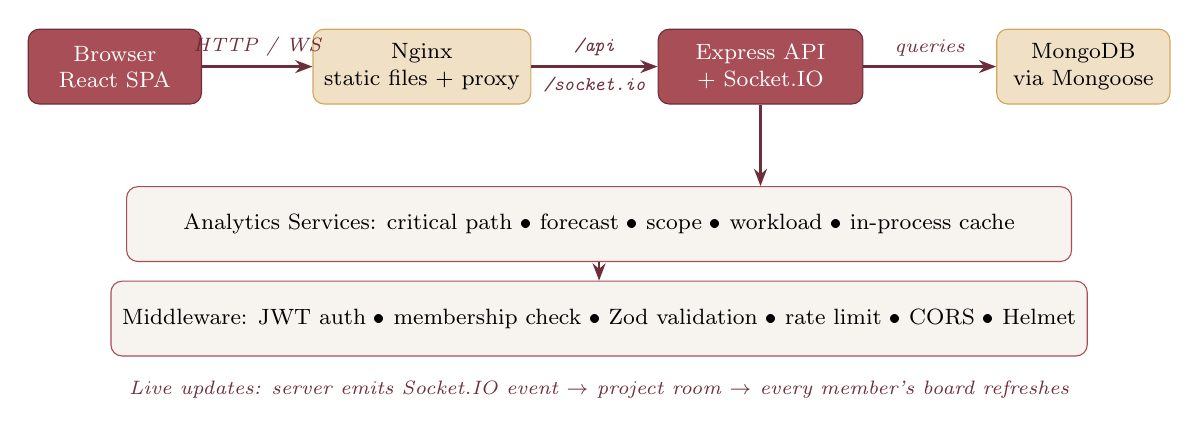
\begin{tikzpicture}
    \node[hot,  minimum width=2.2cm] (spa) at (0,0)    {Browser\\React SPA};
    \node[gold, minimum width=2.4cm] (ng)  at (3.9,0)  {Nginx\\static files + proxy};
    \node[hot,  minimum width=2.6cm] (api) at (8.2,0)  {Express API\\+ Socket.IO};
    \node[gold, minimum width=2.2cm] (db)  at (12.3,0) {MongoDB\\via Mongoose};

    \draw[arr] (spa) -- node[lab, above] {HTTP / WS} (ng);
    \draw[arr] (ng)  -- node[lab, above] {\texttt{/api}} node[lab, below] {\texttt{/socket.io}} (api);
    \draw[arr] (api) -- node[lab, above] {queries} (db);

    \node[box, minimum width=12cm] (svc) at (6.15,-2.0)
      {Analytics Services: critical path \textbullet\ forecast \textbullet\ scope \textbullet\ workload \textbullet\ in-process cache};
    \node[box, minimum width=12cm] (mw) at (6.15,-3.2)
      {Middleware: JWT auth \textbullet\ membership check \textbullet\ Zod validation \textbullet\ rate limit \textbullet\ CORS \textbullet\ Helmet};

    \draw[arr] (api.south) -- (api.south |- svc.north);
    \draw[arr] (svc.south) -- (mw.north);

    \node[lab, align=center] at (6.15,-4.1)
      {Live updates: server emits Socket.IO event $\rightarrow$ project room $\rightarrow$ every member's board refreshes};
  \end{tikzpicture}}
\end{frame}

\begin{frame}{Q3. Data Flow -- Login and Moving a Task}
  \centering
  {\small\bfseries\color{navyMid} (a) Login flow}\\[4pt]
  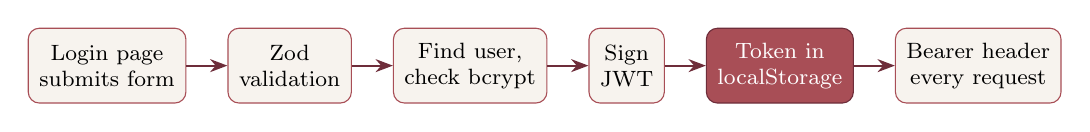
\begin{tikzpicture}[node distance=0.52cm, font=\scriptsize]
    \node[box] (a1) {Login page\\submits form};
    \node[box, right=of a1] (a2) {Zod\\validation};
    \node[box, right=of a2] (a3) {Find user,\\check bcrypt};
    \node[box, right=of a3] (a4) {Sign\\JWT};
    \node[hot, right=of a4] (a5) {Token in\\localStorage};
    \node[box, right=of a5] (a6) {Bearer header\\every request};
    \foreach \x/\y in {a1/a2,a2/a3,a3/a4,a4/a5,a5/a6} \draw[arr] (\x) -- (\y);
  \end{tikzpicture}

  \vspace{0.55cm}
  {\small\bfseries\color{navyMid} (b) Moving a task on the Kanban board}\\[4pt]
  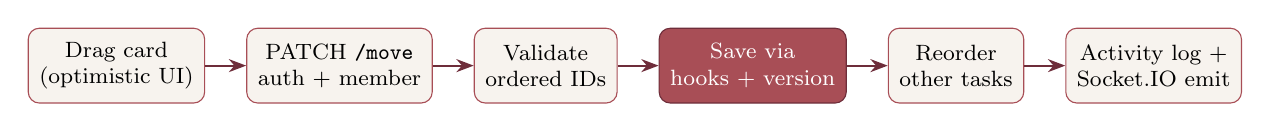
\begin{tikzpicture}[node distance=0.52cm, font=\scriptsize]
    \node[box] (b1) {Drag card\\(optimistic UI)};
    \node[box, right=of b1] (b2) {PATCH \texttt{/move}\\auth + member};
    \node[box, right=of b2] (b3) {Validate\\ordered IDs};
    \node[hot, right=of b3] (b4) {Save via\\hooks + version};
    \node[box, right=of b4] (b5) {Reorder\\other tasks};
    \node[box, right=of b5] (b6) {Activity log +\\Socket.IO emit};
    \foreach \x/\y in {b1/b2,b2/b3,b3/b4,b4/b5,b5/b6} \draw[arr] (\x) -- (\y);
  \end{tikzpicture}

  \vspace{0.4cm}
  \panel[0.9]{\footnotesize\textbf{Key design decision:} the client sends the \emph{full ordered list} of card IDs in the destination column, not just one card's new index. This prevents ordering conflicts when two people drag simultaneously.}
\end{frame}

\begin{frame}{Q3. Data Flow -- Viewing a Sprint Forecast}
  \centering
  \resizebox{\textwidth}{!}{%
  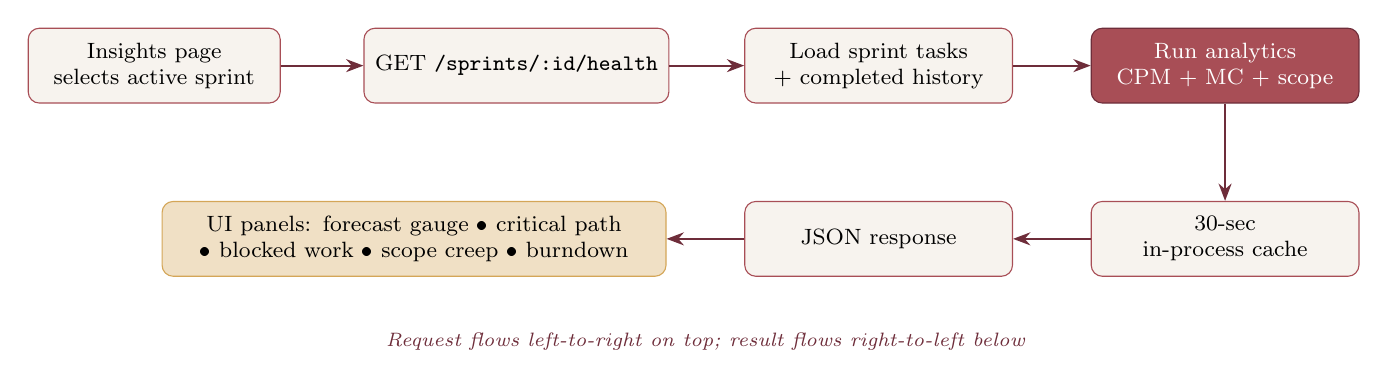
\begin{tikzpicture}[font=\footnotesize]
    \node[box, minimum width=3.2cm] (c1) at (0,0)    {Insights page\\selects active sprint};
    \node[box, minimum width=3.6cm] (c2) at (4.6,0)  {GET \texttt{/sprints/:id/health}};
    \node[box, minimum width=3.4cm] (c3) at (9.2,0)  {Load sprint tasks\\+ completed history};
    \node[hot, minimum width=3.4cm] (c4) at (13.6,0) {Run analytics\\CPM + MC + scope};

    \node[box, minimum width=3.4cm] (c5) at (13.6,-2.2) {30-sec\\in-process cache};
    \node[box, minimum width=3.4cm] (c6) at (9.2,-2.2)  {JSON response};
    \node[gold, minimum width=6.4cm, text width=6cm] (c7) at (3.3,-2.2)
      {UI panels: forecast gauge \textbullet\ critical path \textbullet\ blocked work \textbullet\ scope creep \textbullet\ burndown};

    \draw[arr] (c1) -- (c2);
    \draw[arr] (c2) -- (c3);
    \draw[arr] (c3) -- (c4);
    \draw[arr] (c4) -- (c5);
    \draw[arr] (c5) -- (c6);
    \draw[arr] (c6) -- (c7);

    \node[lab] at (7.0,-3.5) {Request flows left-to-right on top; result flows right-to-left below};
  \end{tikzpicture}}
\end{frame}

\begin{frame}{Q3. Data Model (7 Collections)}
  \centering
  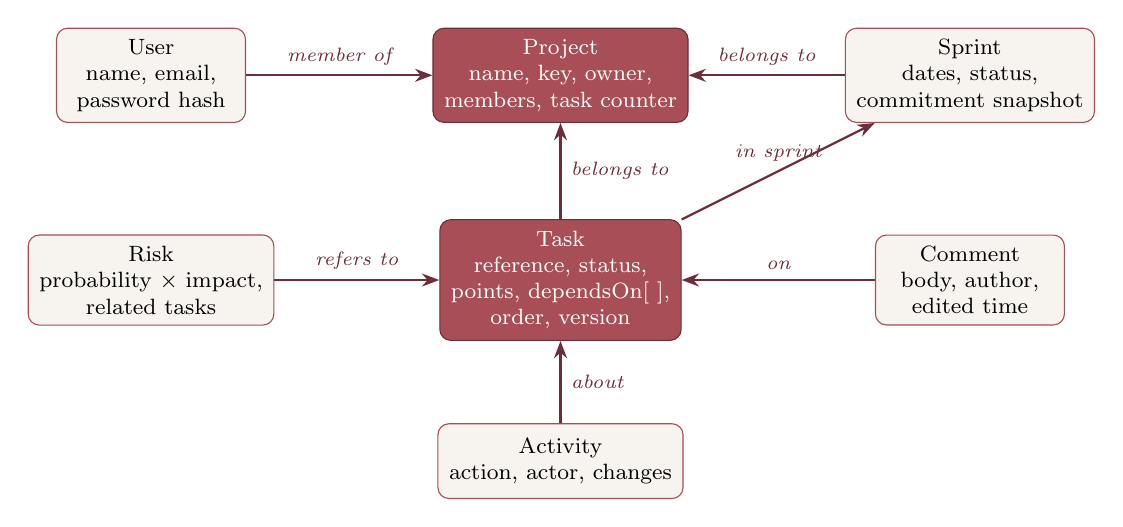
\begin{tikzpicture}[font=\scriptsize]
    \node[hot, minimum width=2.4cm] (proj) at (0,0)    {Project\\name, key, owner,\\members, task counter};
    \node[box, minimum width=2.4cm] (user) at (-5.2,0) {User\\name, email,\\password hash};
    \node[box, minimum width=2.4cm] (spr)  at (5.2,0)  {Sprint\\dates, status,\\commitment snapshot};
    \node[hot, minimum width=2.6cm] (task) at (0,-2.6) {Task\\reference, status,\\points, dependsOn[ ],\\order, version};
    \node[box, minimum width=2.4cm] (risk) at (-5.2,-2.6) {Risk\\probability $\times$ impact,\\related tasks};
    \node[box, minimum width=2.4cm] (com)  at (5.2,-2.6) {Comment\\body, author,\\edited time};
    \node[box, minimum width=2.4cm] (act)  at (0,-4.9)  {Activity\\action, actor, changes};

    \draw[arr] (user) -- node[lab, above] {member of} (proj);
    \draw[arr] (spr)  -- node[lab, above] {belongs to} (proj);
    \draw[arr] (task) -- node[lab, right] {belongs to} (proj);
    \draw[arr] (task) -- node[lab, above] {in sprint} (spr);
    \draw[arr] (risk) -- node[lab, above] {refers to} (task);
    \draw[arr] (com)  -- node[lab, above] {on} (task);
    \draw[arr] (act)  -- node[lab, right] {about} (task);
  \end{tikzpicture}
\end{frame}

\begin{frame}{Q3. API Overview (all routes under \texttt{/api})}
  \footnotesize
  \begin{tabular}{@{}>{\bfseries\color{navyMid}}p{2.6cm}p{6.6cm}p{4.2cm}@{}}
    \toprule
    Area & Routes & Access \\
    \midrule
    Auth & \texttt{POST /auth/register}, \texttt{/login}, \texttt{GET /auth/me} & Public / token \\
    Projects & CRUD + member add/remove & Member; owner for changes \\
    Sprints & CRUD + \texttt{/burndown} & Project member \\
    Tasks & CRUD, \texttt{/move}, dependency add/remove & Project member \\
    Analytics & \texttt{/health}, \texttt{/critical-path}, \texttt{/forecast}, \texttt{/scope-creep}, \texttt{/estimation-accuracy}, \texttt{/workload} & Project member \\
    Collaboration & Comments CRUD, activity log & Member; author for edits \\
    Risks & CRUD under \texttt{/projects/:id/risks} & Project member \\
    System & \texttt{/health}, \texttt{/openapi.json}, \texttt{/docs} & Public \\
    \bottomrule
  \end{tabular}
\end{frame}

% =====================================================================
% ALGORITHMS
% =====================================================================
\begin{frame}{Analytics Engine -- How the Predictions Work}
  \footnotesize
  \begin{tabular}{@{}>{\bfseries\color{navyMid}}p{2.9cm}p{7.0cm}p{3.6cm}@{}}
    \toprule
    Algorithm & Plain-English behaviour & File \\
    \midrule
    Critical Path (CPM) & 3-colour DFS cycle check; Kahn's topological sort; forward and backward passes to get earliest/latest times and float; zero-float tasks form the critical chain & \texttt{criticalPath.js} \\[4pt]
    Monte Carlo forecast & Resample team's historical daily output 5,000 times; count on-time finishes; seeded PRNG (Mulberry32) for reproducibility; reports P50/P85/P95 bands & \texttt{forecast.js} \\[4pt]
    Scope-creep detection & Diff current task list against the commitment snapshot frozen at sprint activation; flag silent point re-estimation & \texttt{scopeAnalysis.js} \\[4pt]
    Estimation accuracy & Compare estimated vs.\ actual story points on done tasks; compute bias ratio and suggest calibration multiplier & \texttt{scopeAnalysis.js} \\[4pt]
    Workload analysis & Group sprint tasks by assignee: load, blocked, overdue, done & \texttt{teamAnalytics.js} \\
    \bottomrule
  \end{tabular}
\end{frame}

% =====================================================================
% Q4 -- CHALLENGES
% =====================================================================
\begin{frame}{Q4. Technical Challenges and Solutions}
  \footnotesize
  \begin{tabular}{@{}>{\color{navyMid}}p{5.1cm}p{8.8cm}@{}}
    \toprule
    \textbf{Challenge} & \textbf{Solution} \\
    \midrule
    Duplicate task references on concurrent creation &
      Atomic counter increment on Project + unique (project, reference) compound index \\
    Dependency cycles break the CPM algorithm &
      3-colour DFS detector; cycle-creating dependency rejected at the API with HTTP 400 \\
    Board reordering skipped Mongoose save hooks &
      Only the moved task goes through \texttt{.save()}; order updates to others use \texttt{bulkWrite} \\
    Removed members kept receiving live events &
      Socket users tracked per room; evicted on membership removal \\
    Forecast was non-repeatable and ignored idle days &
      Keep zero-output days in samples, count working days, use seeded Mulberry32 PRNG \\
    API tests needed a real database &
      \texttt{node:test} + Supertest + \texttt{mongodb-memory-server} -- no external DB required \\
    \bottomrule
  \end{tabular}
  \vspace{0.2cm}
  \panel[0.9]{\footnotesize Each challenge was reproduced in an isolated test, fixed, and covered by a regression test.}
\end{frame}

% =====================================================================
% RESULTS
% =====================================================================
\begin{frame}{Results and Evidence}
  \begin{columns}[T]
    \begin{column}{0.46\textwidth}
      \begin{block}{Automated tests (server)}
        \Large\centering\textbf{77 / 77} \normalsize passing\\[2pt]
        \footnotesize 10 suites, 0 failures.\\Covers analytics, auth, projects, tasks, comments, sprints, validation, concurrency, pagination, and socket eviction.
      \end{block}
      \begin{block}{Codebase size}
        \footnotesize
        \begin{tabular}{@{}lrr@{}}
          Folder & Files & Lines \\ \midrule
          \texttt{server/src}   & 39 & 3,787 \\
          \texttt{server/tests} &  4 & 1,341 \\
          \texttt{client/src}   & 21 & 3,003 \\
        \end{tabular}
      \end{block}
    \end{column}
    \begin{column}{0.50\textwidth}
      \begin{block}{Forecast benchmark (Node v24.2.0)}
        \footnotesize
        \begin{tabular}{@{}rrr@{}}
          \toprule
          Trials & Points remaining & Median time \\ \midrule
          1,000  & 40  & 0.59 ms \\
          5,000  & 40  & 0.95 ms \\
          5,000  & 200 & 1.90 ms \\
          20,000 & 40  & 1.99 ms \\
          50,000 & 40  & 5.66 ms \\
          \bottomrule
        \end{tabular}\\[4pt]
        \scriptsize Production uses 5,000 trials --- sub-millisecond on typical sprints.\\
        Seeded repeatability check: same inputs $\Rightarrow$ same forecast every time.
      \end{block}
    \end{column}
  \end{columns}
\end{frame}

% =====================================================================
% APPLICATION SCREENSHOTS
% =====================================================================
\begin{frame}{Application Screens}
  \begin{columns}[T]
    \begin{column}{0.32\textwidth}\centering
      \shot[0.98]{screenshots/projects.png}{Projects list}\\[3pt]
      {\scriptsize\bfseries\color{navyMid} Projects dashboard}
    \end{column}
    \begin{column}{0.32\textwidth}\centering
      \shot[0.98]{screenshots/board.png}{Kanban board}\\[3pt]
      {\scriptsize\bfseries\color{navyMid} Kanban board}
    \end{column}
    \begin{column}{0.32\textwidth}\centering
      \shot[0.98]{screenshots/planning.png}{Sprint planning}\\[3pt]
      {\scriptsize\bfseries\color{navyMid} Sprint planning}
    \end{column}
  \end{columns}
\end{frame}

\begin{frame}{Delivery Insights and Risk Register}
  \begin{columns}[T]
    \begin{column}{0.32\textwidth}\centering
      \shot[0.98]{screenshots/insights-forecast.png}{Forecast gauge and P50/P85/P95 bands}\\[3pt]
      {\scriptsize\bfseries\color{navyMid} Delivery forecast}
    \end{column}
    \begin{column}{0.32\textwidth}\centering
      \shot[0.98]{screenshots/insights-critical-path.png}{Critical path and burndown}\\[3pt]
      {\scriptsize\bfseries\color{navyMid} Critical path \& burndown}
    \end{column}
    \begin{column}{0.32\textwidth}\centering
      \shot[0.98]{screenshots/risks.png}{Risk register heatmap}\\[3pt]
      {\scriptsize\bfseries\color{navyMid} Risk register}
    \end{column}
  \end{columns}
  \vspace{0.3cm}
  \panel[0.95]{\footnotesize
    \textbf{What the forecast panel shows:}\ Probability of on-time delivery \textbullet\
    P50 / P85 / P95 confidence bands \textbullet\ Critical chain of zero-slack tasks \textbullet\
    Scope growth since sprint commitment \textbullet\ Risk exposure (probability $\times$ impact)}
\end{frame}

% =====================================================================
% Q5 -- LIMITATIONS AND FUTURE SCOPE
% =====================================================================
\begin{frame}{Q5. Limitations of the Current System}
  \begin{columns}[T]
    \begin{column}{0.52\textwidth}
      \begin{itemize}\small
        \item \textbf{Token storage:} JWT kept in \texttt{localStorage}; not revocable on logout
        \item \textbf{Roles:} only \texttt{owner} and \texttt{member}; no fine-grained permissions
        \item \textbf{Forecast calendar:} weekdays only -- no holiday or leave calendar
        \item \textbf{Single instance:} in-process cache and rate-limit; not shared across API replicas
        \item \textbf{New teams:} Monte Carlo needs past sprint history; falls back to estimates for teams with no history
      \end{itemize}
    \end{column}
    \begin{column}{0.44\textwidth}
      \begin{itemize}\small
        \item \textbf{UI coverage:} workload and dependency-graph API endpoints exist but are not surfaced in the UI
        \item \textbf{Health check:} reports process status; does not verify MongoDB connectivity
        \item \textbf{Testing:} 77 server tests; zero client-side automated tests
        \item \textbf{Validation:} benchmarked against seeded demo data, not a real team's history
      \end{itemize}
    \end{column}
  \end{columns}
\end{frame}

\begin{frame}{Q5. Future Scope}
  \begin{columns}[T]
    \begin{column}{0.48\textwidth}
      \begin{block}{Planned (in the project README)}
        \begin{itemize}\small
          \item Cumulative-flow and cycle-time diagrams
          \item What-if simulation: ``drop this task $\Rightarrow$ probability goes to X\%''
          \item Sprint-health alerts when forecast drops below threshold
          \item Roles beyond owner and member
        \end{itemize}
      \end{block}
    \end{column}
    \begin{column}{0.48\textwidth}
      \begin{block}{Natural next steps}
        \begin{itemize}\small
          \item Holiday-aware, per-team working calendar
          \item Workload and dependency-graph views in the UI
          \item Shared Redis cache + rate-limit for multi-instance deployment
          \item Frontend component and end-to-end tests (Playwright)
          \item Calibrate forecasts against real team history
        \end{itemize}
      \end{block}
    \end{column}
  \end{columns}
\end{frame}

% =====================================================================
% THANK YOU
% =====================================================================
\begin{frame}[plain]
  \begin{tikzpicture}[remember picture,overlay]
    \fill[navyDeep] (current page.south west) rectangle (current page.north east);
    \fill[tealAccent] ([yshift=-1.1cm]current page.north west) rectangle
                      ([yshift=-1.18cm]current page.north east);
    \fill[tealAccent] ([yshift=1.0cm]current page.south west) rectangle
                      ([yshift=1.08cm]current page.south east);
  \end{tikzpicture}
  \vfill
  \begin{center}
    {\color{white}\Huge\bfseries Thank You\par}
    \vspace{0.4cm}
    {\color{tealAccent}\large Questions?\par}
    \vspace{0.6cm}
    
\begin{tikzpicture}
      \node[fill=navyMid, rounded corners=6pt, inner sep=8pt, text=white, align=center]{%
        \small Mrunal Nikam \quad Akshit Kumar \quad Bhargavi Piridi};
    \end{tikzpicture}
    \vspace{0.3cm}
    {\color{white}\footnotesize Department of Computer Science \& Engineering\par}
    {\color{white}\footnotesize Indian Institute of Information Technology, Vadodara\par}
    \vspace{0.3cm}
    {\color{tealAccent}\footnotesize\texttt{github.com/bhargavi-46/Predictive-Sprint-Planning}\par}
  \end{center}
  \vfill
\end{frame}

\end{document}
